\section{Especificación del diseño}
Teniendo en cuenta los anteriores requisitos y los objetivos del proyecto la especificación del diseño concretará como se han diseñado las diferentes funcionalidades y como se ha implementado el Federated Learning en el proyecto. Para ello se dividirá el capitulo en las siguientes secciones: Arquitectura, Datos, Modelo de aprendizaje federado.
% \\ \\
% En primer lugar se describirá la arquitectura del proyecto, tanto la configuración de los dispositivos como el como se interconectan y comunican entre sí.  
% En segundo lugar se explicará como se han generado los datos sintéticos y cómo y para que se han utilizado.
% Por último lugar se especificará el modelo de aprendizaje federado, donde se describirán tanto el protocolo de entrenamiento como el protocolo de comunicación.  
% \newpage

% \subsection{Arquitectura}
Es este apartado se explicarán los componentes que toman parte en la arquitectura, como se deben conectar para emular una red de aprendizaje federado y el propio montaje físico de los dispositivos. De esta forma, se podrá comprender porque se han seleccionado los dispositivos que van a participar en el aprendizaje federado, cual es el mapa de red de una red de aprendizaje federado, como se va a representar localmente y como queda el montaje de todos los dispositivos acorde al mapa ded red.  

\subsubsection{Componentes}
Para la recreación de un ejemplo real de una red de aprendizaje distribuido se han utilizado dispositivos de capacidad de computo acotada como son las Raspberry Pi. De esta forma, se pretende demostrar la viabilidad de la aplicación del aprendizaje federado a campos como el del internet de las cosas, donde los dispositivos participantes disponen de escasa capacidad de computo.
\\ \\
De la misma forma, con el objetivo de demostrar que no se necesita un supercomputador para realizar una agregación de modelos, se ha utilizado la NVIDIA Jetson Nano como núcleo central para ello.
\\ \\
Los dispositivos que se utilizarán en concreto son los siguientes: (x4) Raspberry Pi 3 B+ (Fig. \ref{fig:RaspBerrryBPlus}), (x1) NVIDIA Jetson Nano 2GB (Fig. \ref{fig:JetsonNano2GB}) y (x1) Genius switch (Fig. \ref{fig:Switch}).

\begin{figure}[H]
    \begin{minipage}[t]{0.49\linewidth}  % <---
        \centering
        \includegraphics[height=0.1\textheight]{Figuras/Raspberry_Pi_3_B+.png}
        \caption{Raspberry Pi 3 B+ \\ (Fuente: Wikipedia\autocite{ArchivoRaspberryPi})} 
        \label{fig:RaspBerrryBPlus}
    \end{minipage}
    \hfill
    \begin{minipage}[t]{0.5\linewidth}  % <---
        \centering
        \includegraphics[height=0.1\textheight]{Figuras/nvidia_jetson_nano_2GB.png}    
        \caption{NVIDIA Jetson Nano 2GB \\ (Fuente: NVIDIA\autocite{JetsonNano})} 
        \label{fig:JetsonNano2GB}
    \end{minipage}
\end{figure}
\begin{figure}[H]
    \centering
    \includegraphics[height=0.1\textheight]{Figuras/genius_switch.jpg}    
    \caption{Switch Genius} 
    \label{fig:Switch}
\end{figure}
\newpage

\subsubsection{Mapa de red}
Las conexiones entre los dispositivos que interactúan en la red (Raspberrys y Jetson Nano) será por cable, conectando todos al mismo switch para permitir la comunicación entre ellos. A su vez, este switch se conectará al router que proveé de acceso a internet, permitiendo así que los ordenadores de la red puedan acceder a estos dispositivos y estos dispositivos puedan conectarse a internet para lo que necesiten. Todo ello queda representado en el mapa de de la figura \ref{fig:MapaRed}, que sería el mapa de red físico del que parte el proyecto.
\begin{figure}[H]
    \centering
    \includegraphics[width=\textwidth]{Figuras/Network_map.png}    
    \caption{Mapa de red física} 
    \label{fig:MapaRed}
\end{figure}

Esta arquitectura de red lo que permite es que desde el ordenador 1 se pueda acceder a cualquier dispositivo mediante ssh para su configuración y simulación. A su vez, estos dispositivos permanecen físicamente separados los unos de los otros mientras mantienen acceso a internet para realizar tareas de descarga de paquetes, actualizaciones, envío de datos, etc. En este caso, para la transferencia de archivos y ficheros se utilizará el protocolo scp, ya que no entra dentro del alcance el desarrollo de ningún sistema de comunicación y el protocolo scp es fácilmente combinable con el protocolo ssh.

\pagebreak

Sin embargo, desde el punto de vista de la red de aprendizaje federado que quiere simular, el mapa de red incluiría los siguientes cambios:
\begin{itemize}
    \item Cada participante tendría su propia red de área local.
    \item La conexión al servidor de agregación se haría a través de internet.
    \item Los participantes no tendrían ninguna conexión ni relación entre sí.
\end{itemize}
De este modo, el mapa de la red de aprendizaje federado representado en el proyecto quedaría acorde a la figura \ref{fig:FLMapaRed}, aunque el mapa de red sobre el que se opere físicamente sea el de la figura \ref{fig:MapaRed}.

\begin{figure}[H]
    \centering
    \includegraphics[width=0.8\textwidth]{Figuras/FL_network_map.png}    
    \caption{Mapa de la red de aprendizaje federado} 
    \label{fig:FLMapaRed}
\end{figure}

\pagebreak

\subsubsection{Montaje físico}
Una vez realizados todos los mapas y diagramas para la configuración de la red se procedió a conectar los dispositivos acorde al mapa de red físico (fig. \ref{fig:MapaRed}). Para este montaje se acoplaron las Raspberrys que representan a los participantes en el rack mencionado en la sección de gestión de riesgos \ref{GestionRiesgos} mencionada en este mismo capítulo. Despues de conectar todos los cables el montaje quedó como se puede ver en la siguientes imagenes.
\begin{figure}[H]
    \centering
    \begin{minipage}[t]{0.49\linewidth}  % <---
        \includegraphics[height=0.2\textheight]{Figuras/jetsonnano.jpg}
        \caption{Montaje de la Jetson Nano} 
    \end{minipage}
    \hfill
    \begin{minipage}[t]{0.5\linewidth}  % <---
        \includegraphics[height=0.2\textheight]{Figuras/switch.jpg}
        \caption{Montaje del switch} 
    \end{minipage}

    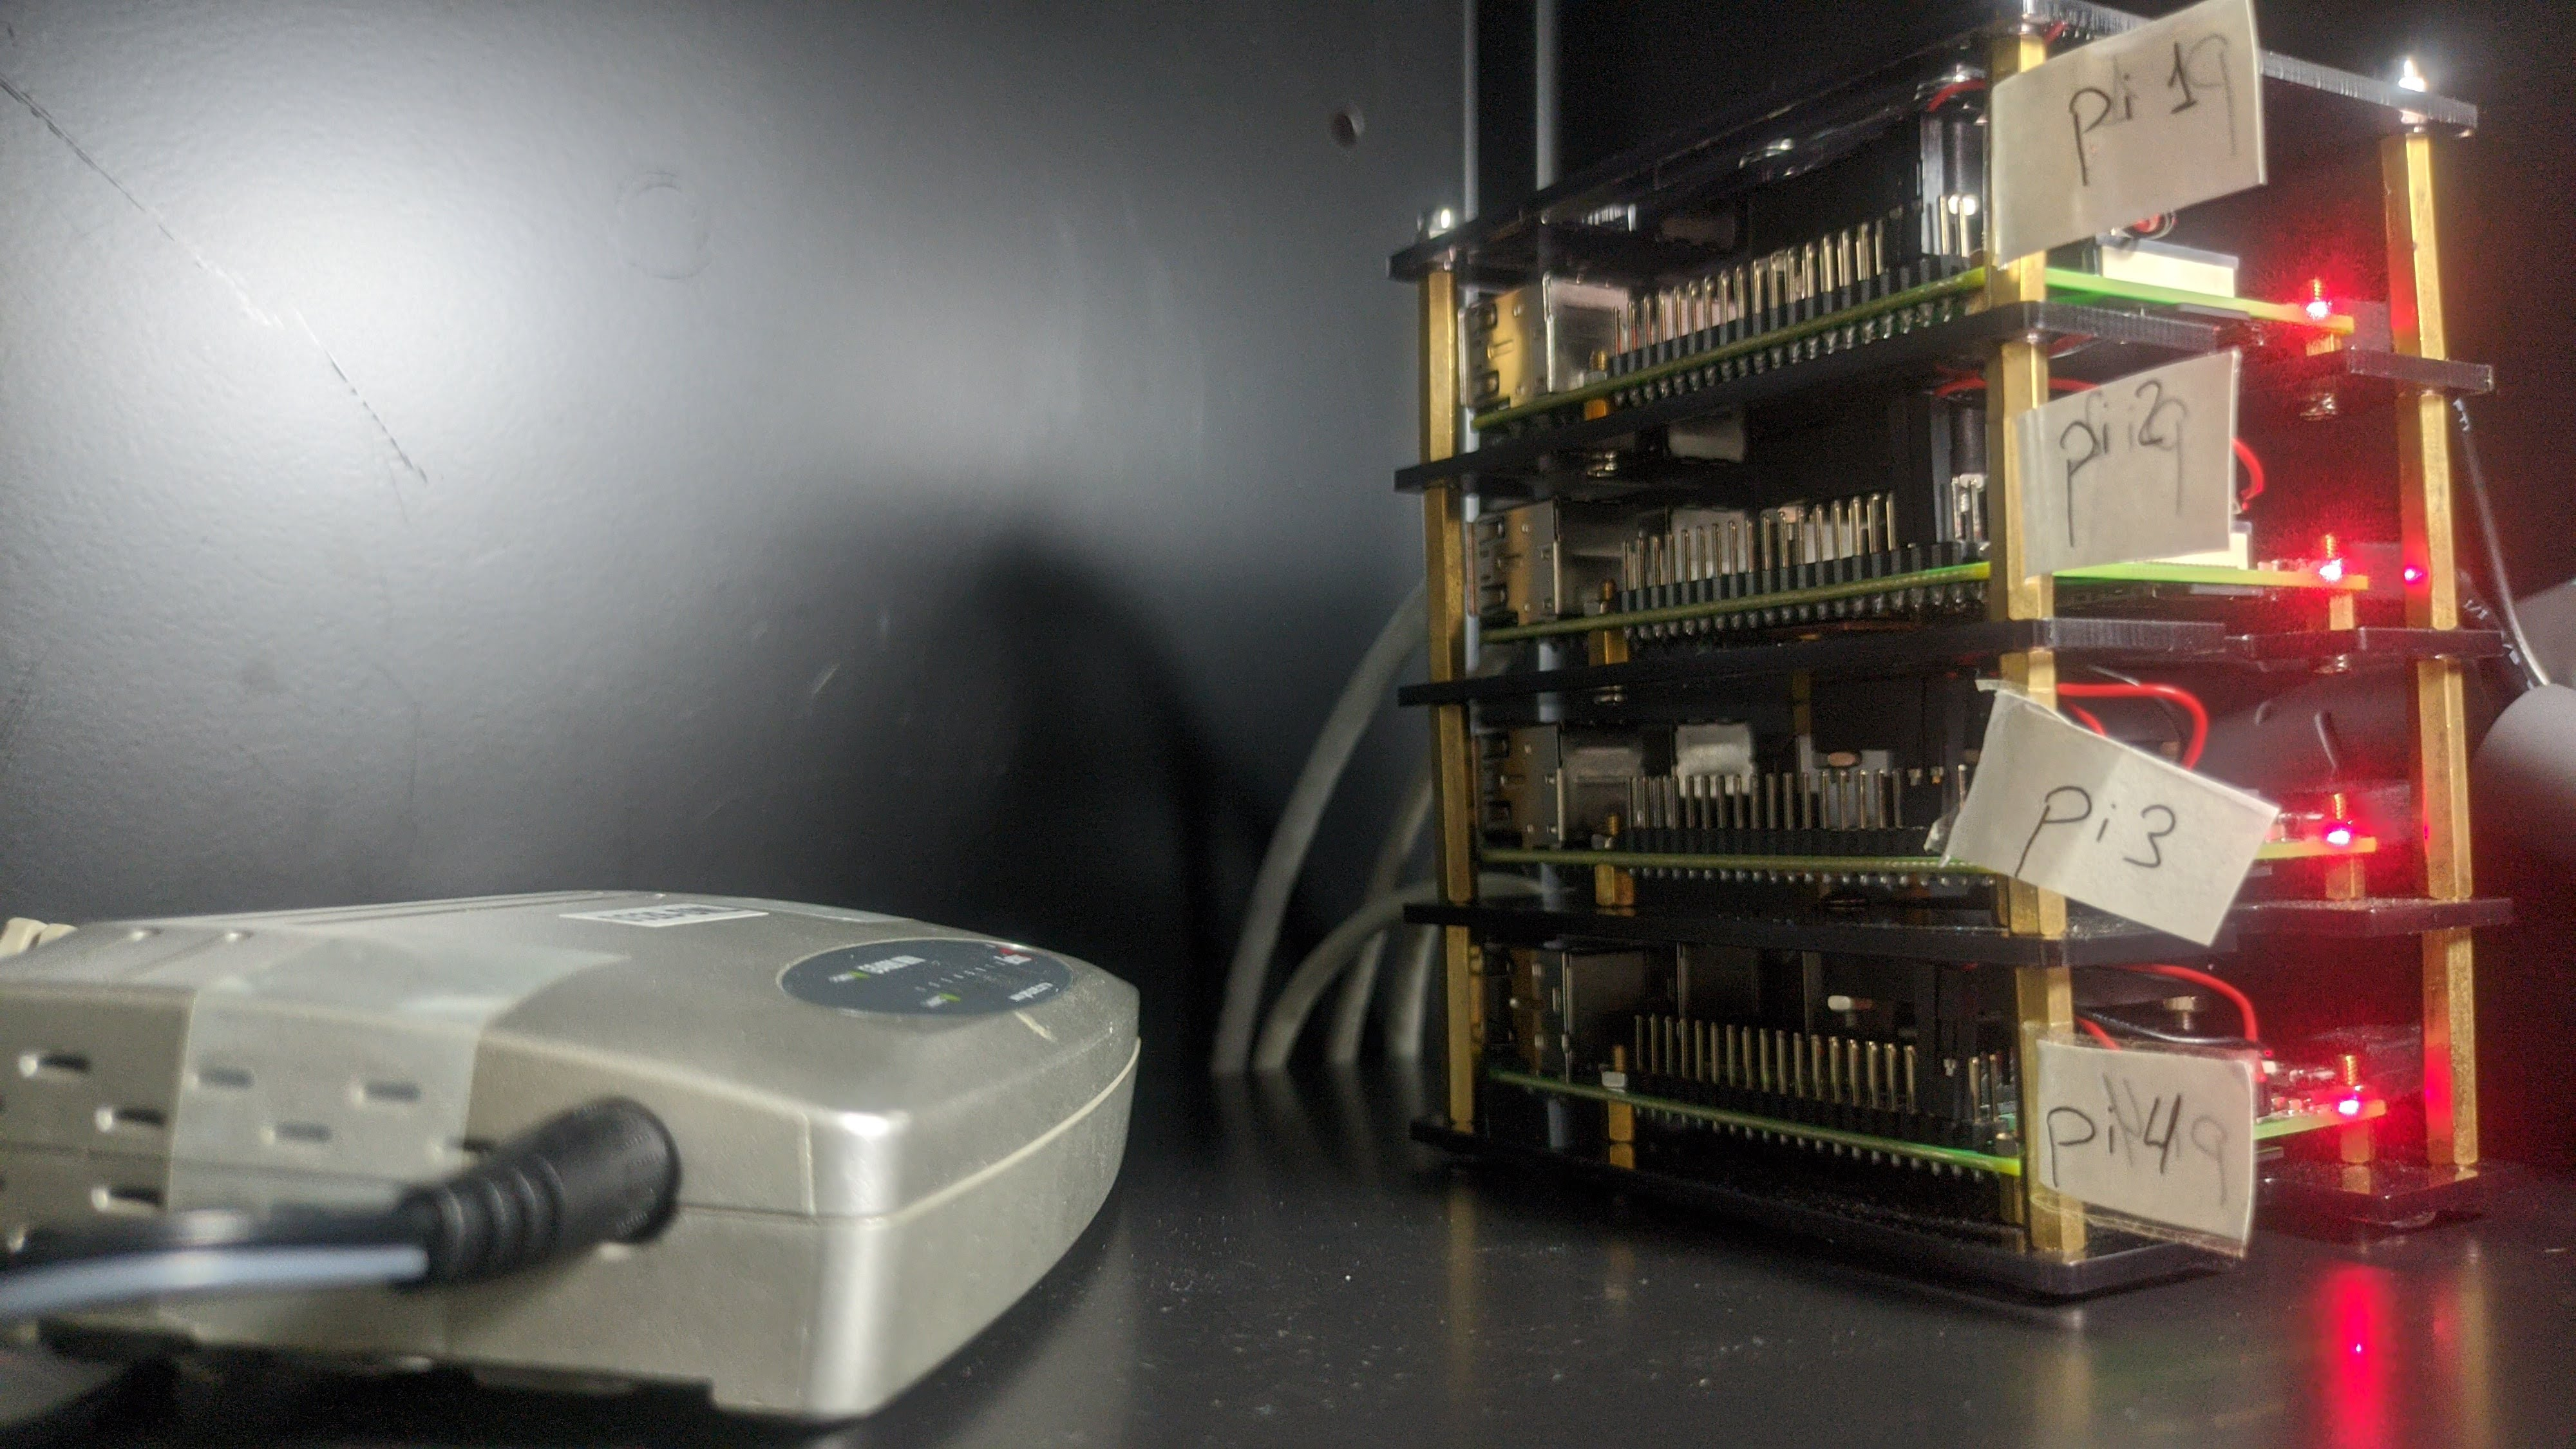
\includegraphics[width=0.75\textwidth]{Figuras/raspberrys.jpg}
    \caption{Montaje de las raspberrys}     
\end{figure}

La Jetson Nano y cada Raspberry tienen un cable ethernet conectado al switch, el cual a su vz cuenta con otro cable ethernet por el cual se conecta al router (no presente en las fotos).


% \newpage

% \subsection{Datos involucrados}
Al tratarse este proyecto de una modificación del sistema de recomendación de R.Sánchez y col., se heredarán todos los datos. Cabe mencionar que R.Sánchez y col. utilizaron información proporcionada por el proyecto Green Soul\autocite{EcoawarePersuasiveNetworked} para crear su sistema de recomendación. El proyecto Green Soul trataba de persuadir a los usuarios para que aumentase su conciencia energética y cambiaran sus hábitos de consumo, para ello, se realizaron una serie de encuestas donde se les preguntaba a los usuarios por sus datos personales y se les pedía que ordenarán en función de su criterio qué estrategias de persuasión les parecían más efectivas.
\\ \\
Por tanto, las estrategias de persuasión que se recomiendan pertenecen al ámbito de la concienciación del consumo energético, aunque podrían ser extrapolables a otros casos. De todas formas, se eludirán los detalles sobre estas estrategias ya que no son el caso de estudio y no entran en el alcance de este proyecto.
\\ \\
Teniendo en cuenta todo lo anterior, este capítulo se ha redactado para entender la gestión de los datos en este proyecto, ya que algunos son de carácter personal y es de suma importancia preservar su privacidad. Estos datos se pueden dividir en tres categorías:
\begin{itemize}
    \item \textbf{No sensibles}, la información de los elementos a recomendar, que no son ni personales ni suministrados por ninguna persona.
    \item  \textbf{Sensibles}, datos que hacen referencia a información personal o que son proporcionados por las personas involucradas en el cuestionario.
    \item \textbf{Sintéticos}, datos de usuarios generados aleatoriamente para paliar la necesidad de datos personales del modelo de consenso (sección \ref{Consenso}.Agregación de modelos por consenso).
\end{itemize} 

\subsubsection{No sensibles}
Como se ha mencionado antes, en la categoría de datos no sensibles se encuentran los datos que no son personales ni hacen referencia a ningún usuario. En esta categoría únicamente aparecen aquellos datos que hacen referencia a los elementos que se van a recomendar en el sistema y sus atributos.
\\ \\
Cada estrategia de persuasión que pueda recomendar el RS contará con hasta dos atributos, para que de esta forma, el sistema pueda conocer mejor las estrategias y realizar recomendaciones más precisas en base a esta información. En la tabla \ref{tab:EstrategiasPersuasion} se muestran las estrategias de persuasión involucradas en el RS y sus atributos.
\begin{table}[H]
    %Con esta función se inicia el entorno tabla, que se puede posicionar con respecto al texto al igual que una imagen.
    
    \begin{center}
    %Se centra la tabla.
        \begin{tabular}{|c|p{0.45\linewidth}|p{0.2\linewidth}|p{0.2\linewidth}|}
            % -------------
            \hline
            \rowcolor{Cyan} 
            % -------------
            \textbf{ID} & \textbf{Descripción} & \textbf{Atributo 1} & \textbf{Atributo 2} \\ 
            % -------------
            \hline
            \textbf{V2} &  Reconocimiento público/social de mi contribución al ahorro de energía. & Reconocimiento social & -\\
            % -------------
            \hline
            \rowcolor{GrisTabla}
            \textbf{V5} & Recibir información relacionada con la energía de una forma simple y estéticamente atractiva. & Atractivo físico & -\\
            % -------------
            \hline
            \textbf{V6} &  Recibir beneficios como recompensa por mejorar mi rendimiento energético(horarios de trabajo flexibles, saltarse ciertas tareas, etc.). & Condicionamiento & -\\
            % -------------
            \hline
            \rowcolor{GrisTabla} 
            \textbf{V7} & Recibir un reconocimiento por lograr ahorros de energía de manera colectiva yo y mi equipo. & Reciprocidad & Reconocimiento social\\
            % -------------
            \hline
            \textbf{V10} & Mis altos gerentes están comprometidos con el ahorro de energía. & Autoridad & Demostración social \\
            % -------------
            \hline
            \rowcolor{GrisTabla} 
            \textbf{V11} & Poder monitorear mi propio desempeño energético en tiempo real. & Monitorización propia. & - \\ 
            % -------------
            \hline
            \textbf{V15} &  Información sobre el efecto que mis acciones pueden tener sobre el consumo de energía. & Causa efecto & -\\
            % -------------
            \hline
            \rowcolor{GrisTabla} 
            \textbf{V17} & Evacuación comparativa de mi desempeño en el ahorro de energía respecto a usuarios parecidos a mí. & - & -\\
            % -------------
            \hline
            \textbf{V19} &  Consejos y sugerencias sobre el ahorro de energía al día o a la semana.  & Sugerencia & -\\
            % -------------
            \hline
            \rowcolor{GrisTabla} 
            \textbf{V20} &  Avances y consejos sobre las lecciones aprendidas de usuarios parecidos mí en acciones específicas de ahorro de energía. & Similaridad & -\\
            \hline

            % \rowcolor{Naranja} 
            % \textbf{V} & \textbf{elit} \\ \hline
        \end{tabular}
        \caption{\centering Estrategias de persuasión del sistema (Fuente: Elaboración propia).}
        \label{tab:EstrategiasPersuasion}
    \end{center}    
\end{table}


\subsubsection{Sensibles}
En cuanto a los datos sensibles hay que mencionar dos grupos, los datos personales de los usuarios y los rankings de los usuarios. Este primer grupo está formado por los datos personales de los usuarios participantes, que intervienen en dos puntos clave: en el entrenamiento de los modelos de IA y a la hora de agregar estos modelos. El grupo de los datos de los rankings está formado por las preferencias de los anteriores usuarios a la hora de ordenar las estrategias de persuasión, es decir, el ranking de estrategias para cada usuario.
\\ \\
Tanto los datos personales de los usuarios como los datos de los rankings de estos son necesarios para entrenar un modelo de IA. Los atributos de los usuarios, al igual que los atributos de las estrategias de persuasión, sirven para relacionar los distintos usuarios entre sí y encontrar relación entre sus diferentes atributos con el orden que le han dado a las diferentes estrategias de persuasión, de esta forma, se pueden realizar recomendaciones en base al tipo de usuario.

\paragraph{Datos de usuarios\\}
Los datos personales de los usuarios que intervienen en este proyecto son los presentes en la tabla \ref{tab:AtributosUsuarios}. Estos datos han sido transformados a objetos json para su posterior utilización, formando una lista de objetos en los que cada uno representa los datos personales de un usuario.
\begin{table}[H]
    %Con esta función se inicia el entorno tabla, que se puede posicionar con respecto al texto al igual que una imagen.
    
    \begin{center}
    %Se centra la tabla.
        \begin{tabular}{|c|c|p{0.7\linewidth}|}
            % -------------
            \hline
            \rowcolor{Cyan} 
            % -------------
            \textbf{ID} & \textbf{Nombre} & \textbf{Descripción}\\ 
            % -------------
            \hline
            \textbf{0} &  Edad & Rango de edad\\
            % -------------
            \hline
            \rowcolor{GrisTabla}
            \textbf{1} & Género & Género\\
            % -------------
            \hline
            \textbf{2} & Educación & Nivel educativo\\
            % -------------
            \hline
            \rowcolor{GrisTabla} 
            \textbf{3} & País & País de residencia\\
            % -------------
            \hline
            \textbf{4} & Cultura de trabajo & Cultura de trabajo\\
            % -------------
            \hline
            \rowcolor{GrisTabla} 
            \textbf{5} & PST & Tipo de perfil de usuario en base a los propuestos por Dan Lockton\autocite{locktonModelsUserDesigners2012} : \textit{"Pinball, Shortcut, Thought-ful"}\\ 
            % -------------
            \hline
            \textbf{6} & Barreras  & Barreras ante el cambio\\
            % -------------
            \hline
            \rowcolor{GrisTabla} 
            \textbf{7} & Intenciones & Intenciones ante el cambio\\
            % -------------
            \hline
            \textbf{8} & Confianza  & Confianza ante el cambio\\
            % -------------
            \hline

            % \rowcolor{Naranja} 
            % \textbf{V} & \textbf{elit} \\ \hline
        \end{tabular}
        \caption{\centering Atributos de los usuarios que participan en el sistema (Fuente: Elaboración propia).}
        \label{tab:AtributosUsuarios}
    \end{center}    
\end{table}
\paragraph{Rankings\\}
Los usuarios, a parte de introducir sus datos personales anteriores, también introducen el orden de las estrategias de persuasión en base a la relevancia que consideran que tienen. Este ranking de estrategia es recogido y transformado a formato json formando una lista de objetos json en la que cada objeto representa los datos de la tabla \ref{tab:RankingUsuario}.
\begin{table}[H]
    \begin{center}
    %Se centra la tabla.
        \begin{tabular}{|c|p{0.7\linewidth}|}
            % -------------
            \hline
            \rowcolor{Cyan} 
            % -------------
            \textbf{Nombre} & \textbf{Descripción}\\ 
            % -------------
            \hline
            \textbf{User ID}  & Identificador único del usuario\\
            % -------------
            \hline
            \rowcolor{GrisTabla}
            \textbf{Item ID}  & Identificador único de la estrategia de persuasión\\
            % -------------
            \hline
            \textbf{Ranking} & Valor en el ranking de la estrategia de persuasión\\
            % -------------
            \hline
            % \rowcolor{Naranja} 
            % \textbf{V} & \textbf{elit} \\ \hline
        \end{tabular}
        \caption{\centering Elementos de la estructura de los datos del ranking  (Fuente: Elaboración propia).}
        \label{tab:RankingUsuario}
    \end{center}    
\end{table}


\subsubsection{Sintéticos}
En cuanto a los datos sintéticos, se debe tener en cuenta que los datos sensibles han sido directamente suministrados por los usuarios, por lo cual, es técnicamente imposible acceder a ellos desde el servidor de agregación, ya que sería una evidente violación de la privacidad de los usuarios. Esto genera un gran problema debido a que el propio modelo de consenso, explicado en la sección \ref{Consenso}, requiere de datos de usuarios para funcionar.
\\ \\
La forma de abordar el problema de la necesidad de datos es mediante la creación de usuarios sintéticos, como se explica en la subsección \ref{Consenso:Usuarios_Sinteticos}. Estos usuarios sintéticos tendrán los mismos atributos que los usuarios normales (tabla \ref{tab:AtributosUsuarios}), tendrán que clasificar las mismas estrategias de persuasión (tabla \ref{tab:EstrategiasPersuasion}) y el ranking se gestionará de la misma forma (tabla \ref{tab:RankingUsuario}).


% \newpage

% \subsection{Protocolo de Federated Learning}\label{Protocolo}
El protocolo de Federated Learning que se va a reproducir en este proyecto es una adaptación de lo que proponen K. Bonawitz y col. \autocite{bonawitzFederatedLearningScale2019a}. En este protocolo se definen tres fases importantes, la selección de participantes, la configuración del mecanismo de agregación y el envío reporte de cada participante.
\\\\
Para este caso se han introducido leves cambios en este protocolo que se irán explicando en las sucesivas partes del mismo.  

\subsubsection{Selección de participantes}
La selección de participantes al tratarse de un caso de estudio concreto no se limita ni se controla de ninguna forma, simplemente se ha implementado una red en la que participan cuatro dispositivos diferentes.

\subsubsection{Intercambio de claves}
El intercambio de claves es una de las novedades introducidas sobre el protocolo previamente mencionado, en este paso, el objetivo es que los diferentes dispositivos de la red compartan sus claves públicas para poder asegurar la privacidad de la red, imagen \ref{fig:PublicKeyShare}. 
\\ \\
La utilización de estas claves públicas y su función están definidas en el apartado de securización de las comunicaciones \ref{SegCom}.
\begin{figure}[H]
    \centering
    \includegraphics[width=0.5\textwidth]{Figuras/Network_public_key.png}    
    \caption{Intercambio de claves públicas entre los participantes} 
    \label{fig:PublicKeyShare}
\end{figure}

\subsubsection{Entrenamiento}
El entrenamiento es algo que en el protocolo se omite pero que es importante mencionar. Este proceso se lleva a cabo en el dispositivo del participante y conlleva dos tareas:
\begin{itemize}
    \item En primer lugar este participante crea su modelo de IA, lo entrena con los datos que él elija y lo almacena.
    \item En segundo lugar este modelo es cifrado y enviado al servidor. El proceso de cifrado se puede observar en el diagrama \ref{fig:Flow_Encryption} de la sección de securización de las comunicaciones \ref{SegCom}.
\end{itemize} 
\begin{figure}[H]
    \centering
    \includegraphics[height=0.6\textheight]{Figuras/flowchart_train.png}    
    \caption{Intercambio de claves públicas entre los participantes} 
    \label{fig:Entrenamiento}
\end{figure}

\subsubsection{Comunicación con el servidor}
La comunicación con el servidor es un proceso crucial en el que se debe asegurar que los modelos de los participantes lleguen sin modificaciones y sin ser interceptados por ningún atacante. Para detallar este proceso se ha elaborado una sección donde se explican más a fondo los pasos llevados para conseguir que las comunicaciones sean seguras, sección \ref{SegCom}.
\\ \\
Debido a este protocolo de seguridad, los participantes deberán enviar tanto los modelos cifrados como las claves cifradas, acorde las siguientes imágenes.

\begin{figure}[H]
    \begin{minipage}[t]{0.45\linewidth}  % <---
        \centering
        \includegraphics[width=\textwidth]{Figuras/Network_participant_encrypted_key.png}
        \caption{Envío de la clave de cifrado del modelo al servidor de agregación} 
    \end{minipage}
    \hfill
    \begin{minipage}[t]{0.45\linewidth}  % <---
        \centering
        \includegraphics[width=\textwidth]{Figuras/Network_participant_encrypted_model.png}    
        \caption{Envío del modelo cifrado al servidor de agregación} 
    \end{minipage}
\end{figure}

\subsubsection{Agregación de los modelos}
En este proceso, como tal, no va a ocurrir una agregación de modelos, sino más bien una compartición de conocimiento de forma indirecta mediante el modelo de consenso. Este sistema está explicado con detalle en la sección \ref{Consenso} de este capítulo.
\\ \\
De todas formas, para verlo de una forma más sencilla, se puede observar el siguiente diagrama \ref{fig:Flow_Agregation} en el cual se muestra el flujo de los datos y de los modelos para ser agregados. El proceso que recorre este diagrama puede ser dividido en 4 partes:
\begin{itemize}
    \item Se reciben los modelos de los participantes (en este caso 4), se descifran siguiendo el diagrama \ref{fig:Flow_Decryption} (explicado con detalle en en la sección de securización de las comunicaciones \ref{SegCom}) y se guardan los modelos para su posterior utilización.
    \item Una vez se cuente con los modelos descifrados, se generan los usuarios sintéticos. Después, con el modelo de cada participante se realiza la predicción del ranking para estos usuarios y se almacena para su posterior utilización. 
    \item Mediante el modelo de consenso explicado en el apartado \ref{Consenso} estas predicciones son convertidas a una única predicción por usuario sintético generado. Después, la información se almacena para su uso final.
    \item Por último, se coge toda la información de los usuarios sintéticos y los rankings consensuados para reentrenar el modelo de cada participante. 
\end{itemize}
\begin{figure}[H]
    \centering
    \includegraphics[width=\textwidth]{Figuras/flowchart_agregation.png}    
    \caption{Diagrama del flujo de reentrenado de los modelos} 
    \label{fig:Flow_Agregation}
\end{figure}
\newpage
\subsubsection{Comunicación con los participantes}
La comunicación del servidor con los participantes se realiza de la misma forma en la que los participantes se comunican con el servidor. La única diferencia es que el receptor en este caso son los participantes y el emisor el servidor.
\begin{figure}[H]
    \begin{minipage}[t]{0.45\linewidth}  % <---
        \centering
        \includegraphics[width=\textwidth]{Figuras/Network_node_encrypted_key.png}
        \caption{Envío de la clave de cifrado del modelo de cada participante a cada participante} 
    \end{minipage}
    \hfill
    \begin{minipage}[t]{0.45\linewidth}  % <---
        \centering
        \includegraphics[width=\textwidth]{Figuras/Network_node_encrypted_model.png}    
        \caption{Envío de cada modelo cifrado a su correspondiente dueño} 
    \end{minipage}
\end{figure}
\subsubsection{Comparación de modelos}
En el momento que el modelo llega al participante, este tiene que valorar si realmente le supone una mejora o no. Para ello como puede verse en el diagrama \ref{fig:Flow_Compare}, existen varias fases a llevar a cabo.

En primer lugar, al igual que como con el servidor de agregación, se debe descifrar el modelo recibido. Después, compararlo con el modelo del participante. Esto se puede hacer tratando de analizar la precisión de las predicciones para varios subconjuntos de datos de test con los que cuente el dispositivo. En resumen, predecir para los usuarios existentes de su ranking con los dos modelos y quedarse con el modelo que más acierte.

\begin{figure}[H]
    \centering
    \includegraphics[height=0.6\textheight]{Figuras/flowchart_compare.png}    
    \caption{Diagrama del flujo de la comparación de los modelos} 
    \label{fig:Flow_Compare}
\end{figure}


% \newpage

% \subsection{Securización de las comunicaciones} \label{SegCom}
Para preservar la seguridad y privacidad durante las comunicaciones del protocolo de FL propuesto es imprescindible securizar las comunicaciones. Para securizar las comunicaciones se han llevado a cabo dos acciones clave, la primera en lo que concierne al protocolo de comunicación y la segunda en cuanto al cifrado de la comunicación.

\subsubsection{Protocolo de comunicación}
En cuanto al protocolo de comunicación, se ha optado por la utilización del protocolo SCP (Secure Copy Protocol), conocido en español como protocolo de copia segura. Este protocolo requiere del protocolo SSH (Secure Shell), conocido en español como terminal seguro.
\\ \\
El protocolo SSH permite el acceso remoto a un servidor o dispositivo por un canal seguro a través de una clave. Además, el protocolo usa técnicas de cifrado que impiden que la información que viaje en la red lo haga de forma legible. El protocolo SCP permite la transferencia de archivos entre dispositivos de la red usando el protocolo SSH como base.

\subsubsection{Cifrado de la comunicación}
Aunque las comunicaciones en el protocolo SCP y SSH vayan cifradas son susceptibles de ser atacadas. Para mejorar este aspecto se ha realizado un sistema de cifrado de los modelos que viajen por la red para preservar la privacidad y seguridad de los participantes.
\\ \\ 
Para esta labor se han utilizado el método criptográfico de criptografía híbrida, que usa tanto la criptografía simétrica como asimétrica.

\paragraph{Cifrado simétrico} 
El cifrado simétrico es aquel sistema de cifrado en el que la misma clave sirve para cifrar como para descifrar el mensaje. 
\\ \\
El problema de este sistema es que toda la seguridad reside en la clave empleada en el cifrado. Esto es un gran impedimento a la hora de gestionar comunicaciones debido al la forma de envíar la clave, ya que, si no se hace por un canal seguro, el mensaje sera fácilmente descifrable.
\\ \\
Por otro lado, este sistema cuenta con dos grandes ventajas, es sencillo, es rápido y requiere menos recursos para llevarlo a cabo.

\paragraph{Cifrado asimétrico}
El cifrado asimétrico es aquel sistema de cifrado que consta de dos claves criptográficas, una pública y una privada. La clave pública es utilizada para cifrar el mensaje, mientras que la privada es utilizada para descifrarlo. 
\\ \\
Este sistema cuenta con tres grandes desventajas que impiden su uso en exclusivo o su uso con grandes volúmenes de información a cifrar. 
\begin{itemize}
    \item Se necesita más procesado de cómputo para generar la clave.
    \item Las claves asimétricas son mucho más grandes que las simétricas.
    \item El mensaje cifrado ocupa más espacio que el original.
\end{itemize}

Debido a que los dispositivos con los que se cuenta no tienen una gran capacidad de cómputo no se podría establecer un tamaño de clave lo suficientemente grande como para poder cifrar el modelo de IA completo. Este modelo, pesa alrededor de los 7Kb y para cifrarlo con este sistema habría que generar una clave del mismo tamaño o mayor.
\\ \\
Sin embargo, este sistema al constar de dos claves independientes es más sencillo de implementar, puesto que no se envía la clave con la que se descifra el mensaje, sino con la que se cifra, lo que facilita la tarea y evita la búsqueda de canales seguros para enviar las cláves.

\paragraph{Cifrado híbrido}
Teniendo en cuenta los anteriores dos tipos de cifrado se decidió utilizar el sistema híbrido para obtener los resultados más óptimos, protegiendo la privacidad y pudiendo realizar las tareas de cifrado desde dispositivos con menor capacidad computacional.
\\ \\ 
El proceso de cifrado se ha realizado de acuerdo al diagrama de flujo representado en la figura \ref{fig:Flow_Encryption}. En este diagrama se pueden observar los pasos que se han realizado para la encriptación de la información, en primer lugar el modelo de LightFM se convirtió a bytes y se comprimió para reducir el volumen de datos a enviar por la red, pudiendo agilizar así las comunicaciones. Después se cifró simétricamente, generando una clave y un mensaje cifrado. Por un lado este mensaje cifrado sería comprimido y se guardaría en un fichero para su posterior envío. Mientras que por el otro lado, la clave de cifrado simétrica se encriptó asimétricamente con la clave pública del receptor del mensaje, dando como resultado una clave de cifrado simétrico cifrada asimétricamente. Esta clave sería guardada en un fichero para ser enviada al igual que el mensaje.
\begin{figure}[H]
    \centering
    \includegraphics[height=0.6\textheight]{Figuras/flowchart_encryption.png}    
    \caption{Diagrama de flujo del proceso de cifrado} 
    \label{fig:Flow_Encryption}
\end{figure}


\subsubsection{Descifrado del mensaje}
El descifrado del mensaje es el proceso inverso al cifrado de la figura \ref{fig:Flow_Encryption}. Para ello, en un primer momento se reciben tanto el modelo cifrado simétricamente como la clave del modelo cifrada asimétricamente. En primer lugar, la clave que se ha recibido se descifra asimétricamente con la clave privada propia, ya que esta sólo es descifrable por el receptor. Una vez descifrada la clave, se descomprime el modelo y se descifra con esta. Por último, el resultado es descomprimido y convertido a objeto LightFM para su posterior utilización. 
\begin{figure}[H]
    \centering
    \includegraphics[height=0.6\textheight]{Figuras/flowchart_decryption.png}    
    \caption{Diagrama de flujo del proceso de descifrado} 
    \label{fig:Flow_Decryption}
\end{figure}

% \newpage


\subsection{Agregación de modelos}\label{Consenso}

\subsubsection{Generar usuarios sintéticos}\label{Consenso:Usuarios_Sinteticos}


\subsubsection{Predecir ranking de los usuarios}

\subsubsection{Consensuar predicciones}

\subsubsection{Generar rankings sintéticos}

\subsubsection{Exportación de datos}

\subsubsection{Reentrenado}